% ============================================================
\chapter{Introduction to Machine Learning}
\label{ch:introduction}
\index{machine learning}
% ============================================================

\section{What is Machine Learning?}

\begin{definition}[Machine Learning]
\textbf{Machine learning} is the study of algorithms that automatically
improve their performance on a given task through experience (data), without
being explicitly programmed for that task~\cite{murphy2022}.
\end{definition}

More formally, following Tom Mitchell: a program learns from experience $E$
with respect to a class of tasks $T$ and a performance measure $P$, if its
performance on $T$, as measured by $P$, improves with experience $E$.

\section{Types of Learning}
\label{sec:types}
\index{learning!types}

\begin{center}
\begin{tikzpicture}[
  cat/.style={rectangle, draw, rounded corners, minimum width=3cm,
    minimum height=1cm, align=center, font=\small\bfseries},
  sub/.style={rectangle, draw, rounded corners, fill=white,
    minimum width=2.8cm, font=\scriptsize, align=center}
]
  \node[cat, fill=blue!15] (sup) {Supervised};
  \node[cat, fill=green!15, right=2.5cm of sup] (unsup) {Unsupervised};
  \node[cat, fill=orange!15, right=2.5cm of unsup] (rl) {Reinforcement};

  \node[sub, below=0.4cm of sup] (s1) {Regression\\Classification};
  \node[sub, below=0.4cm of unsup] (s2) {Clustering\\Dim.\ Reduction};
  \node[sub, below=0.4cm of rl] (s3) {Exploration\\Exploitation};

  \draw[-{Stealth}] (sup) -- (s1);
  \draw[-{Stealth}] (unsup) -- (s2);
  \draw[-{Stealth}] (rl) -- (s3);
\end{tikzpicture}
\end{center}

\subsection{Supervised Learning}
\index{learning!supervised}

We have a dataset $\mathcal{D} = \{(\bm{x}_i, y_i)\}_{i=1}^n$ where
$\bm{x}_i \in \R^d$ is a feature vector and $y_i$ is the label. The goal
is to learn a function $f : \R^d \to \mathcal{Y}$ such that
$f(\bm{x}) \approx y$ for new data.

\begin{itemize}
  \item \textbf{Regression}: $\mathcal{Y} = \R$ (apartment price,
    temperature).
  \item \textbf{Classification}: $\mathcal{Y} = \{1, \ldots, K\}$
    (spam/not-spam, handwritten digits).
\end{itemize}

\subsection{Unsupervised Learning}
\index{learning!unsupervised}

We have only $\mathcal{D} = \{\bm{x}_i\}_{i=1}^n$ without labels. The goal
is to discover hidden structure: clusters, low-dimensional manifolds,
distributions.

\subsection{Reinforcement Learning}
\index{learning!reinforcement}

An agent interacts with an environment, receives rewards, and learns a
policy maximizing cumulative reward. This paradigm is not covered in this
course.

\section{Mathematical Formalization}
\label{sec:formalization}

\subsection{Hypothesis Space}

\begin{definition}[Hypothesis space]
The \textbf{hypothesis space}\index{hypothesis space} $\mathcal{H}$ is the
set of functions $h : \R^d \to \mathcal{Y}$ among which the learning
algorithm searches for the best one.
\end{definition}

\begin{example}[Linear regression]
$\mathcal{H} = \{h_{\bm{w}} : \bm{x} \mapsto \bm{w}^\top \bm{x} + b
\mid \bm{w} \in \R^d, b \in \R\}$.
\end{example}

\subsection{Loss Function and Risk}
\index{loss function}

\begin{definition}[Loss function]
A \textbf{loss function} $\ell : \mathcal{Y} \times \mathcal{Y} \to \R_+$
measures the error between the prediction $\hat{y} = h(\bm{x})$ and the
true value $y$. Common examples:
\begin{align}
  \text{Squared error:} \quad & \ell(y, \hat{y}) = (y - \hat{y})^2 \\
  \text{0-1 error:} \quad & \ell(y, \hat{y}) = \ind[y \neq \hat{y}] \\
  \text{Log-loss:} \quad & \ell(y, \hat{y}) = -y\log\hat{y} - (1-y)\log(1-\hat{y})
\end{align}
\end{definition}

\begin{definition}[Risk]
The \textbf{risk} (or generalization error)\index{risk} of a hypothesis $h$ is:
\begin{equation}
  R(h) = \E_{(\bm{x}, y) \sim P}[\ell(y, h(\bm{x}))]
\end{equation}
where $P$ is the (unknown) joint distribution of the data.
\end{definition}

\begin{definition}[Empirical risk]
The \textbf{empirical risk}\index{risk!empirical} is the approximation of
the risk on the training data:
\begin{equation}
  \hat{R}_n(h) = \frac{1}{n} \sum_{i=1}^n \ell(y_i, h(\bm{x}_i))
\end{equation}
\end{definition}

\begin{keyformulas}[title=\textbf{Empirical Risk Minimization (ERM)}]
The learning algorithm seeks:
\begin{equation}
  h^* = \argmin_{h \in \mathcal{H}} \hat{R}_n(h) = \argmin_{h \in \mathcal{H}}
  \frac{1}{n} \sum_{i=1}^n \ell(y_i, h(\bm{x}_i))
  \label{eq:erm}
\end{equation}
\end{keyformulas}

\section{The Bias-Variance Tradeoff}
\label{sec:bias-variance}
\index{bias-variance}

\begin{theorem}[Bias-variance decomposition]
For the squared loss, the risk decomposes as:
\begin{equation}
  \E[(y - \hat{f}(\bm{x}))^2] = \underbrace{\Bias^2[\hat{f}(\bm{x})]}_{\text{bias}^2}
  + \underbrace{\Var[\hat{f}(\bm{x})]}_{\text{variance}}
  + \underbrace{\sigma^2_\varepsilon}_{\text{irreducible noise}}
\end{equation}
where $\Bias[\hat{f}(\bm{x})] = \E[\hat{f}(\bm{x})] - f(\bm{x})$ and
$\sigma^2_\varepsilon = \Var[\varepsilon]$.
\end{theorem}

\begin{center}
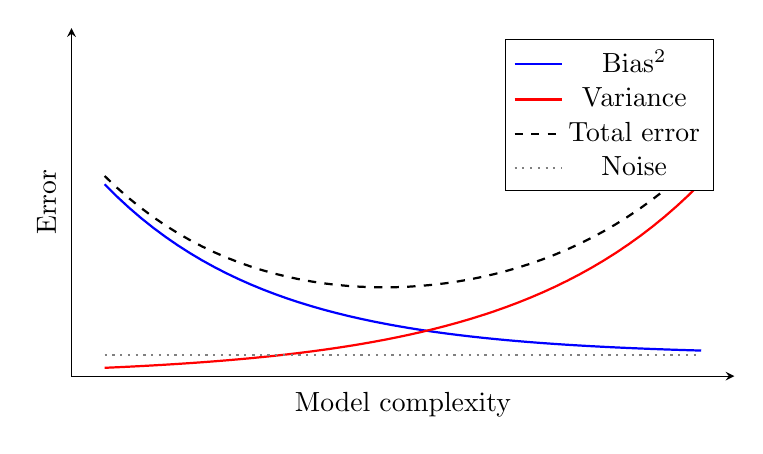
\begin{tikzpicture}
  \begin{axis}[
    width=10cm, height=6cm,
    xlabel={Model complexity},
    ylabel={Error},
    xmin=0, xmax=10, ymin=0, ymax=5,
    legend pos=north east,
    axis lines=left,
    xtick=\empty, ytick=\empty
  ]
    \addplot[thick, blue, domain=0.5:9.5, samples=50] {3*exp(-0.4*x) + 0.3};
    \addlegendentry{Bias$^2$}
    \addplot[thick, red, domain=0.5:9.5, samples=50] {0.1*exp(0.35*x)};
    \addlegendentry{Variance}
    \addplot[thick, black, dashed, domain=0.5:9.5, samples=50]
      {3*exp(-0.4*x) + 0.1*exp(0.35*x) + 0.3};
    \addlegendentry{Total error}
    \addplot[thick, gray, dotted, domain=0.5:9.5] {0.3};
    \addlegendentry{Noise}
  \end{axis}
\end{tikzpicture}
\end{center}

\begin{intuition}[title=\textbf{Interpretation}]
\begin{itemize}
  \item A model that is too simple (high bias) fails to capture the data
    structure: \textbf{underfitting}.
  \item A model that is too complex (high variance) fits the noise:
    \textbf{overfitting}.
  \item The goal is to find the optimal tradeoff.
\end{itemize}
\end{intuition}

\section{Model Evaluation}
\label{sec:evaluation}
\index{evaluation}

\subsection{Data Splitting}

\begin{bestpractice}[title=\textbf{Train / Validation / Test}]
\begin{itemize}
  \item \textbf{Training} (60--80\,\%): to fit the parameters.
  \item \textbf{Validation} (10--20\,\%): to choose hyperparameters.
  \item \textbf{Test} (10--20\,\%): to estimate final performance.
    \textbf{Never} used for model selection.
\end{itemize}
\end{bestpractice}

\subsection{Cross-Validation}
\index{cross-validation}

\begin{definition}[$k$-fold cross-validation]
We partition the data into $k$ subsets (folds). For each fold $i$:
\begin{enumerate}
  \item Train on the remaining $k-1$ folds.
  \item Evaluate on fold $i$.
\end{enumerate}
The cross-validation error is the mean of the $k$ errors:
\begin{equation}
  \text{CV}(k) = \frac{1}{k} \sum_{i=1}^k \hat{R}^{(i)}
\end{equation}
\end{definition}

\subsection{Metrics}

\begin{keyformulas}[title=\textbf{Common metrics}]
\textbf{Regression:}
\begin{align}
  \text{MSE} &= \frac{1}{n}\sum_{i=1}^n (y_i - \hat{y}_i)^2, \quad
  \text{RMSE} = \sqrt{\text{MSE}}, \quad
  R^2 = 1 - \frac{\sum(y_i-\hat{y}_i)^2}{\sum(y_i - \bar{y})^2}
\end{align}

\textbf{Classification:}
\begin{align}
  \text{Precision} &= \frac{TP}{TP + FP}, \quad
  \text{Recall} = \frac{TP}{TP + FN}, \quad
  F_1 = 2 \cdot \frac{\text{Prec.} \times \text{Recall}}{\text{Prec.} + \text{Recall}}
\end{align}
\end{keyformulas}

\section{Implementation: First Model with scikit-learn}
\label{sec:first-model}

\begin{codeblock}[title=\textbf{Iris classification with scikit-learn}]
\begin{minted}{python}
import numpy as np
from sklearn.datasets import load_iris
from sklearn.model_selection import train_test_split, cross_val_score
from sklearn.neighbors import KNeighborsClassifier
from sklearn.metrics import classification_report

# Load data
X, y = load_iris(return_X_y=True)

# Train/test split
X_train, X_test, y_train, y_test = train_test_split(
    X, y, test_size=0.2, random_state=42, stratify=y
)

# k-NN model
model = KNeighborsClassifier(n_neighbors=5)
model.fit(X_train, y_train)

# Evaluation
print(f"Test accuracy: {model.score(X_test, y_test):.4f}")
print(classification_report(y_test, model.predict(X_test)))

# 5-fold cross-validation
scores = cross_val_score(model, X, y, cv=5, scoring="accuracy")
print(f"CV accuracy: {scores.mean():.4f} +/- {scores.std():.4f}")
\end{minted}
\end{codeblock}

\begin{codeoutput}
\begin{verbatim}
Test accuracy: 1.0000
              precision    recall  f1-score   support
           0       1.00      1.00      1.00        10
           1       1.00      1.00      1.00        10
           2       1.00      1.00      1.00        10
    accuracy                           1.00        30
CV accuracy: 0.9667 +/- 0.0211
\end{verbatim}
\end{codeoutput}

\section{Exercises}
\label{sec:exercises-ch1}

\begin{exercise}[Empirical risk]
Let $\mathcal{D} = \{(1, 2), (2, 3.5), (3, 6)\}$ and $h_w(x) = wx$.
\begin{enumerate}
  \item Compute $\hat{R}_3(h_w)$ with the squared loss for $w = 1.5$ and
    $w = 2$.
  \item Find $w^*$ minimizing $\hat{R}_3(h_w)$ analytically.
  \item Plot $\hat{R}_3(h_w)$ as a function of $w$.
\end{enumerate}
\end{exercise}

\begin{exercise}[Bias-variance decomposition]
\begin{enumerate}
  \item Show that $\E[(y - \hat{f})^2] = \Bias^2 + \Var + \sigma^2$,
    detailing each step.
  \item Generate $n = 50$ points with $y = \sin(x) + \varepsilon$,
    $\varepsilon \sim \mathcal{N}(0, 0.3)$. Fit polynomials of degrees
    1, 3, 5, 10, 15 and illustrate the bias-variance tradeoff.
\end{enumerate}
\end{exercise}

\begin{exercise}[Cross-validation]
\begin{enumerate}
  \item Implement $k$-fold cross-validation from scratch (without
    \pkg{sklearn.model\_selection}).
  \item Compare your implementation's results with \cli{cross\_val\_score}
    for k-NN on the Iris dataset.
  \item Study the effect of $k$ (number of neighbours) on CV accuracy.
    Plot the accuracy vs $k$ curve for $k \in \{1, 3, 5, 7, \ldots, 25\}$.
\end{enumerate}
\end{exercise}
